%----------------------------引入宏包---------------------------%
\documentclass[a4paper,transmag,12pt]{IEEEtran}    %transmag 实现双列排版,摘要跨列
\usepackage[utf8]{inputenc}
\usepackage{xeCJK}
\usepackage{graphicx}
\usepackage[justification=centering]{caption}
\usepackage{natbib}     %漂亮的bib引用
\usepackage{bm}         %设置缩进
\usepackage{fancyhdr}   %页眉页脚
\usepackage{chemfig}    %化学方程式
\usepackage{amsmath}    %数学公式阵列
\usepackage{multirow}   %表格合并单元格

%----------------------------设置字体族--------------------------%
\CJKfamily{STFangsong}
\setmainfont{Times New Roman}
\setsansfont{Arial}
%\setCJKmainfont[BoldFont=SimHei]{Noto Sans CJK SC}
%\setCJKmonofont{Noto Mono}

\newcommand{\song}{\CJKfamily{STFangsong}}    % 宋体
\newcommand{\hei}{\CJKfamily{SimHei}}         % 黑体


%------------------------------设置字体大小------------------------%  
\newcommand{\chuhao}{\fontsize{42pt}{\baselineskip}\selectfont}     %初号  
\newcommand{\xiaochuhao}{\fontsize{36pt}{\baselineskip}\selectfont} %小初号  
\newcommand{\yihao}{\fontsize{28pt}{\baselineskip}\selectfont}      %一号  
\newcommand{\erhao}{\fontsize{21pt}{\baselineskip}\selectfont}      %二号  
\newcommand{\xiaoerhao}{\fontsize{18pt}{\baselineskip}\selectfont}  %小二号  
\newcommand{\sanhao}{\fontsize{15.75pt}{\baselineskip}\selectfont}  %三号  
\newcommand{\sihao}{\fontsize{14pt}{\baselineskip}\selectfont}      %四号  
\newcommand{\xiaosihao}{\fontsize{12pt}{\baselineskip}\selectfont}  %小四号  
\newcommand{\wuhao}{\fontsize{10.5pt}{\baselineskip}\selectfont}    %五号  
\newcommand{\xiaowuhao}{\fontsize{9pt}{\baselineskip}\selectfont}   %小五号  
\newcommand{\liuhao}{\fontsize{7.875pt}{\baselineskip}\selectfont}  %六号  
\newcommand{\qihao}{\fontsize{5.25pt}{\baselineskip}\selectfont}    %七号  
%------------------------------标题名称中文化-----------------------------%  
%\renewcommand\abstractname{\hei 摘\ 要}  
%\renewcommand\refname{\hei 参考文献}  
\renewcommand\figurename{\hei 图}  
\renewcommand\tablename{\hei 表}
%\renewcommand\thesection{\textbf{第\arabic{section}章 }}
%\renewcommand\thesubsection{\textbf{第\arabic{section}.\arabic{subsection}节}}
%\renewcommand\thesubsubsection{\textbf{\arabic{section}.\arabic{subsection}.\arabic{subsubsection}}}


%-------------------------------设置页面属性-----------------------------%
\usepackage{indentfirst}
\setlength{\parindent}{2em} %设置自动缩进为两格
\captionsetup{font={small}}     %设置图表标题大小

%-------------------------------设置数学环境-----------------------------%
\setatomsep{2em}    %设置化学键长度

%-------------------------------设置快捷命令-----------------------------%
\newcommand{\cdegree}{$^{\circ}$C}  %摄氏度


%-------------------------------文档部分---------------------------------%
\begin{document}

\title{\sanhao 共聚(丙烯腈-丁二烯)和氯化聚氯乙烯的共混物中的混溶行为}
\author{Wansoo Huh' and Frank E. Karasz' \\
        translated by 朱浩南}
\date{1992}

%设置页眉页脚
\fancyhf{}
\pagestyle{fancy}
\chead{共聚(丙烯腈-丁二烯)和氯化聚氯乙烯的共混物中的混溶行为}
\fancyfoot[C]{\thepage}
%双线页眉的设置
\makeatletter %双线页眉
\def\headrule{{\if@fancyplain\let\headrulewidth\plainheadrulewidth\fi%
\hrule\@height 1.0pt \@width\headwidth\vskip1pt%上面线为1pt粗
\hrule\@height 0.5pt\@width\headwidth  %下面0.5pt粗
\vskip-2\headrulewidth\vskip-1pt}      %两条线的距离1pt
\vspace{6mm}}     %双线与下面正文之间的垂直间距
\makeatother


\IEEEtitleabstractindextext{
\begin{abstract}
摘要——研究了氯化聚氯乙烯(CPVC)和共聚(丙烯腈-丁二烯)(AN-BT)共聚物的 50/50 wt\% 共混物的混溶性和相行为。通过利用差示扫描量热法测量,确定了在 150\cdegree 下的混溶性-不混溶性边界。发现与 PVC/(AN-BT) 系统相比,CPVC/(AN-BT)系统的混溶度随 CPVC 氯含量的增加而变大。在 CPVC 共混体系中,最大混溶性区域发现约为 63 wt\% 的Cl。通过假设两个组分的无规共聚物结构,并将一阶均匀场理论应用于实验结果,确定了相互作用参数 $\chi_{ij}$'s。理论相边界与实验数据一致。通过研究温度对该共混物的相行为的影响,确定了较低的临界溶液温度行为,如 170\cdegree 下的混溶性区域的收缩。
\end{abstract}
}

\maketitle
\IEEEdisplaynontitleabstractindextext
\IEEEpeerreviewmaketitle


\section{介绍}
在聚合物-聚合物共混物中的混溶性行为已经被研究了 30 多年,部分是为了开发具有所需材料性质的新型聚合物体系。找到新的可混溶聚合物体系的这些努力仍在进行中,因为相对较少的聚合物共混物表现出热力学相容性。通常当两种组分之间存在有利的特异性相互作用(如氢键,偶极相互作用或离子相互作用)时,含有高分子量聚合物的混合物的混合体系具有较好的相容性。就目前的体系而言,Prud'homme、Paul 和他的同事们研究了 CPVC 与芳族聚酯,聚己内酯和聚(甲基丙烯酸烷基酯)共混物的混溶行为。他们发现氯代聚合物中氯含量高(48-56\% 质量分数 Cl)以及需要聚酯和聚甲基丙烯酸酯中的最佳 \chemfig{CH_2}/COO 比来获得最大的双酚二磷相互作用,这导致热力学相互作用的值为负,因此具有混溶性。\par{}
根据最近开发的聚合物混合理论,如状态方程或格子流体理论,Gibbs 混合自由能含有三个贡献:混合的组合熵,交换相互作用和自由体积效应。对于高分子量材料的混合物,组合熵项是可忽略的,并且对于可混溶系统需要负交换相互作用。然而,其中至少一种组分由无规共聚物组成的一些聚合物共混物已经被发现在某些共聚物组成范围内是可混溶的,即使相应的均聚物的二元组合中没有一种是可混溶的。没有确定这些系统的特异性分子间相互作用。由于包含该共聚物的两种不同单体单元之间的所谓的排斥相互作用,产生“混溶性窗口”。类型 $\rm{(A_{1-x}B_x)_n/C_m}$ 的可混溶体系的实例是聚氯乙烯/共聚(乙烯-乙酸乙烯酯),聚甲基丙烯酸甲酯/共聚(苯乙烯-丙烯腈)和其它含聚苯醚(PPO)的共混体系。由 $\rm{(A_{1-x}B_x)_n/(C_{1-y}D_y)_m}$ 所示类型的共聚物共聚物体系,共聚(丁二烯-苯乙烯)/共聚(氯乙烯-乙酸乙烯酯)与其它共聚物共聚物共混物含有磺化聚苯氧基(SPPO)的体系的系统显示了一定范围的共聚物组合物的混溶性。在这种情况下,需要表示四种不同单体单元的二元组合的六个分段相互作用参数来描述无规共聚物-共聚物混合物的相行为。混合的自由能由下式给出
\begin{equation}
    \begin{aligned}
        \varDelta G/RT = &(\phi_1/N_1)ln\phi_1 + (\phi_2/N_2)ln\phi_2 + \\
                          &\phi_1\phi_2(1-x)(1-y)\chi_{AC} + y(1-y)\chi_{AD} + \\
                          &x(1-y)\chi_{BC} + xy\chi_{BD} - x(1-x)\chi_{AB} - \\
                          &y(1-y)\chi_{CD})
    \end{aligned}
\end{equation}

在平均场近似中,其中 x 和 y 是共聚物摩尔组成,$\phi_1$和$\phi_2$是两个组分的体积分数。$N_1$和$N_2$表示各共聚物的聚合度,$\chi_{ij}$'s表示相应的分段相互作用参数。 通过利用 ten Brinke 等人的方法,如果确定所有相互作用参数,则可以获得两种共聚物混合物之间的等温相界。\par{}
对于由 Shiomi 等人研究的 CPVC 与共聚(乙烯-乙酸乙烯酯)的混合物,通过平均场方法预测的相图显示与实验结果良好的一致性。Kang、Karasz和 MacKnight 使用平均场理论对磺化聚苯醚与其他共聚物体系的共混物的相行为研究。他们从独立获得的分段相互作用参数$\chi_{ij}$'s计算了共聚物共混物的相边界。 发现实验结果与平均场理论的预测吻合良好。\par{}
在我们的实验室,已经做了大量的努力来了解含氯化共聚物的混合物的复相行为。最近对氯化聚乙烯(CPE)与不同氯含量的共混物的研究表明,混合窗口的最大值在约 50 wt\% 的氯含量下发生。这些系统显示氯含量低于 50 wt\% 的较高临界溶解温度(UCST)类型行为和低于 50 wt\% 氯含量的临界溶解温度(LCST)型行为。\par{}

\begin{table*}[!htbp]
    \caption{PVC 氯含量}
    \label{tab:}
    \begin{center}
        \begin{tabular}{cccccc}
             \hline
             CPVC Cl, wt\% & CPVC $\rm{T_g}$ & \chemfig{CH_2CHCl} mol \% & CHClCHCl mol \% & \chemfig{CHClCCl_2} mol \% & \chemfig{CH_2CCl_2} mol \% \\
             \hline
             56.7   &85.5   &100.0(0.0) &0.0    &0.0    &0.0    \\
             59.0   &91.0   &90.0(10.0) &8.2    &0.3    &1.5    \\
             61.9   &103.8  &77.4(22.6) &18.9   &0.7    &3.0    \\
             62.3   &107.5  &75.3(24.7) &20.2   &1.2    &3.3    \\
             63.7   &113.2  &68.3(31.7) &25.5   &2.1    &4.1    \\
             64.4   &121.3  &64.8(35.2) &28.1   &2.6    &4.5    \\
             65.5   &138.8  &59.0(41.0) &32.0   &3.8    &5.2    \\
             66.5   &143.9  &53.1(46.9) &35.1   &6.0    &5.8    \\
             67.1   &146.4  &49.4(50.6) &36.8   &7.8    &6.0    \\
             68.1   &157.0  &41.1(58.9) &41.4   &11.0   &6.5    \\
             68.5   &162.3  &37.8(62.2) &43.0   &12.4   &6.8    \\
             \hline
        \end{tabular}
    \end{center}
\end{table*}

聚氯乙烯(PVC)与共聚(丙烯腈-丁二烯)(AN-BT)的混溶性已经得到广泛的研究:Matsuo 和同事们研究了 PVC/(AN-BT) 的粘弹性和形态。 Zakrzewski 报道,PVC和 (AN-BT) 共聚物的共混物中的混溶窗在丙烯腈组合物的共聚物组成范围为 23-45 wt\% 之间发生。 在该范围内,通过差示扫描量热法(DSC),动态力学分析(DMA)和电子显微镜来表示单相均匀结构。 使用流变学测量,广角X射线分析,光散射分析和透射电子显微镜(TEM)揭示了混溶性 PVC/(AN-BT) 系统的类似结果。\par{}
在本研究中,氯化聚氯乙烯(CPVC)被视为由 \chemfig{CH_2CHCl} 和 \chemfig{CHClCHCl} 单元组成的无规共聚物,而 PVC 被认为是交替共聚物。通过改变两种共聚物的显微组织和化学组成,使用平均场理论研究和解释了相行为。

\section{实验部分}
从 B.F.Goodrich 公司得到 Geon 103-EP 级(Mw = 209000 和 Mn = 136000)的聚(乙烯-1氯化物)。氯化聚氯乙烯通过溶液氯化制备;通过改变反应停留时间控制氯含量。通过元素分析(马萨诸塞大学微量分析实验室)测定 CPVC 的化学成分。表 I 列出氯重量百分比和所有 \chemfig{CH_2-CHCl},CHClCHCl,\chemfig{CHClCCl_2},\chemfig{CH_2CCl_2} mol\%。所有共聚(丙烯腈-丁二烯)(AN-BT)(Mw = 180,000)共聚物均得自 Scientific Polymer Products Inc.,除了 10 和 16 AN mol\%(AN-BT)共聚物, BF Goodrich Co.使用九种不同(AN-BT)共聚物组合物,其范围为10-51 AN mol\%。 通过GPC测定所有分子量,并对流体动力学体积进行校正。CPVC 分子量测量表明在氯化过程中基本上不存在降解。\par{}
通过将 (AN-BT) 和 PVC 或 CPVC 溶解在常用溶剂 THF 中制备共混物;将混合物搅拌数天,沉淀成十倍以上的甲醇。两种聚合物的混合比例为 50/50(重量比)。将沉淀的样品用新鲜甲醇洗涤数次以除去剩余的 THF,然后在 65\cdegree 下干燥 3 天。\par{}
通过使用 Perkin-Elmer DSC-4 差示扫描量热仪观察玻璃化转变来研究共混物的混溶性。$\rm{T_g}$是根据 $dC_p/dT$ 对温度的最大值的位置确定的,其中 $\rm{C_p}$ 是热容量。将样品在 DSC 中在特定温度下退火 15 分钟,然后淬灭至低于较低组分 $\rm{T_g}$ 的温度。 加热速率为 20\cdegree/min。

\begin{figure}[!htbp]
    \centering
    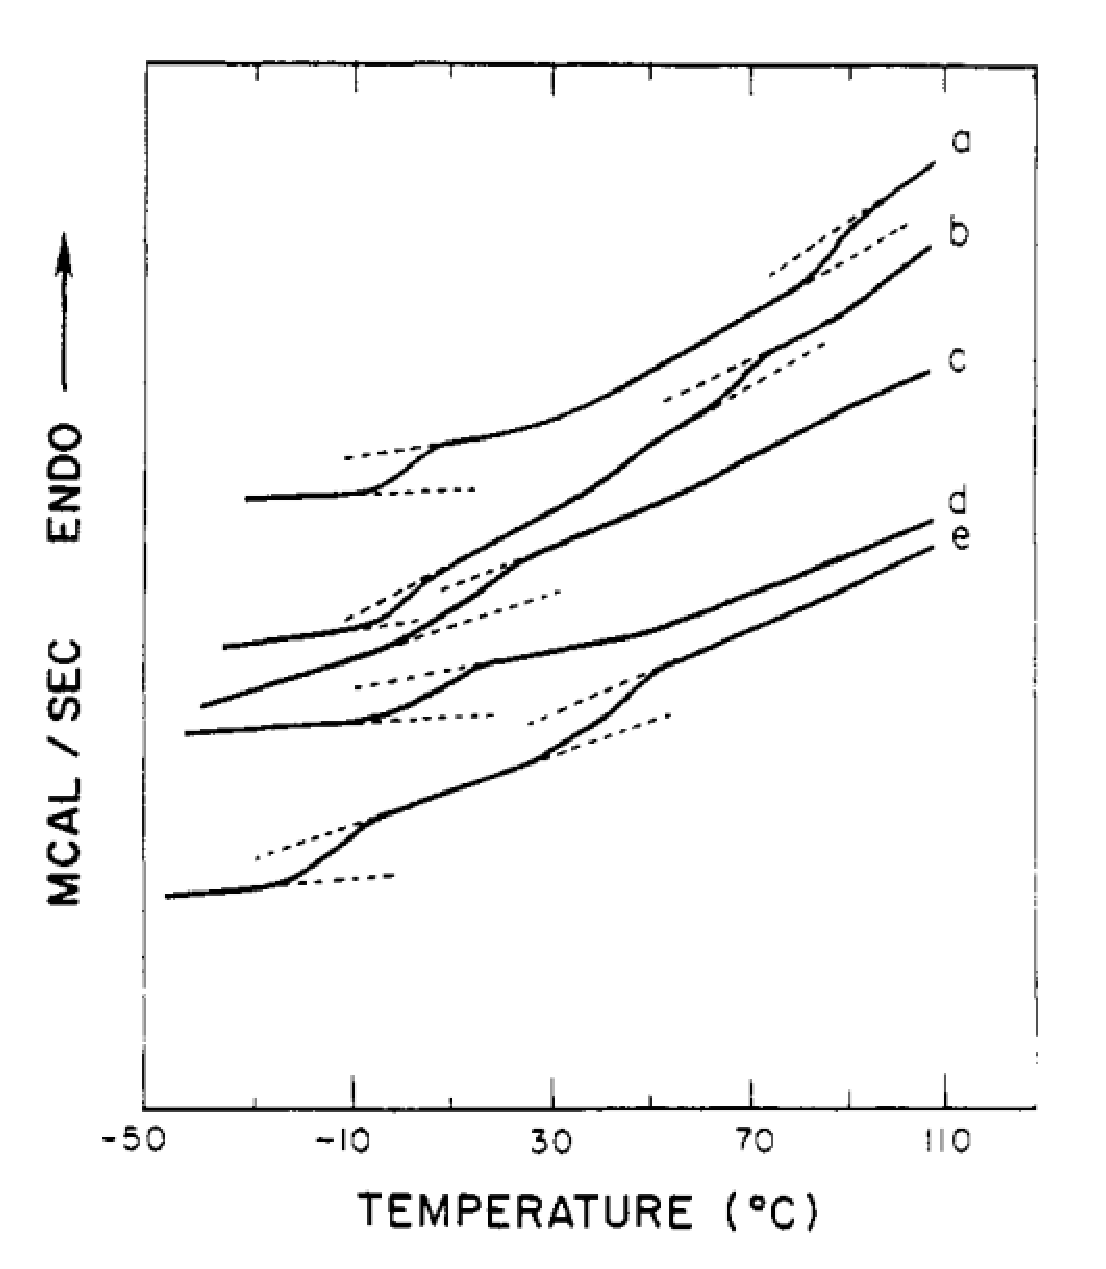
\includegraphics[width=.9\linewidth]{src/figure1.eps}
    \caption{PVC/(AN-BT) 混合物的差示扫描量热法测定图:(a) PVC/(51\% AN-BT);(b) PVC/(44\% AN-BT);(c) PVC/(33\% AN-BT);(d)PVC/(27\% AN-BT);(e) PVC/(20\% AN-BT)}
\end{figure}

\section{结果与讨论}
聚氯乙烯的 $T_g$ 为 85.5\cdegree,氯含量为 56.7 wt\%。氯化可增加 CHCl 单元的数量并增加 $T_g$,如表 I 所示。例如,含有 68.1 wt\% Cl (CPVC-9) 的 CPVC 的 $T_g$ 为 157\cdegree,而 CPVC 的 $T_g$ 为 59 wt\% 的 Cl (CPVC-1) 为 91\cdegree。如表 I 所示,CPVC 包含 \chemfig{CH_2 CHCl},\chemfig{CHClCHCl},以及 \chemfig{CHClCCl_2} 和 \chemfig{CH_2CCl_2} 单元,其取决于氯化水平。从 \chemfig{^{13}C} NMR 结果可以看出,与较低氯化水平的其他单元相比,\chemfig{CCl_2} 单元的存在较小。作为近似值,CPVC 可以表示为 $(A_{1-x}B_x)_n$,其中 A 是 PVC 组分(\chemfig{CH_2CHCl}单元),B 是包含 CHClCHCl,\chemfig{CHClCCl_2} 和 \chemfig{CH_2CCl_2} 单位的组分。这里,x 是重复单元 B 的摩尔分数,n 是聚合度。(AN-BT)共聚物由丙烯腈(AN)和丁二烯(BT)单元组成,随机排列,可以表示为 $(C_{1-y}D_y)_m$,其中 \chemfig{C~BT},\chemfig{D~AN},y 是摩尔重复单元 D 的分数,m 是聚合度。通过独立地将 x 和 y 从 0 变化到 1,可以改变 CPVC/(AN-BT) 共混体系的组成。\par{}
图 I 显示了在 150\cdegree 退火 15 分钟的 PVC/(AN-BT)混合物的 DSC 热分析图;AN-BT 共聚物的 AN 含量为 20~51 mol\%。含有 27 和 33 mol\% AN 含量的共混物显示典型的可混溶行为,如单一 $T_g$,而含有 20,44 和 51 的 AN mol\% 的其它体系表现出与纯 PVC 和 (AN-BT)共聚物不同的 $T_g$。\par{}

\begin{figure}[!htbp]
    \centering
    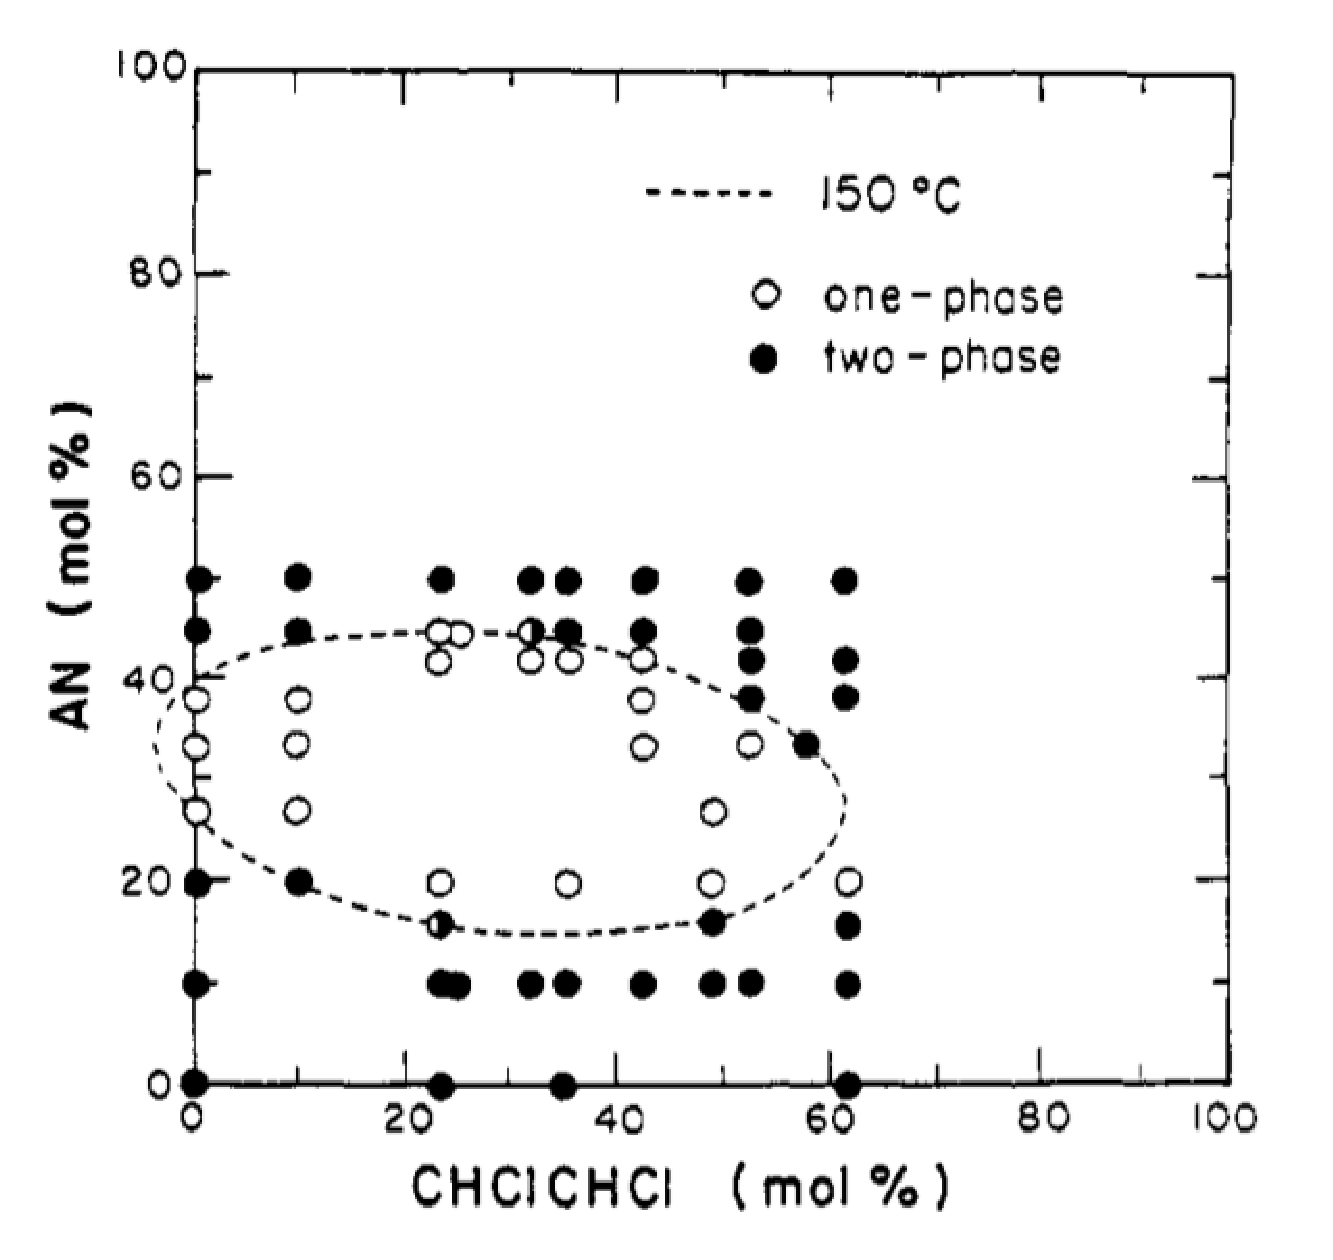
\includegraphics[width=.9\linewidth]{src/figure2.eps}
    \caption{150\cdegree 时 CPVC/(AN-BT) 共混物的等温混溶性-不混溶性图。半虚圆表示不明确的分配。}
\end{figure}

\begin{table}[!htbp]
    \caption{计算 150 和 170\cdegree 的相互作用参数}
    \label{tab:}
    \begin{center}
        \begin{tabular}{ccc}
             \hline
             \multirow{2}{*}{结构单元对} &\multicolumn{2}{c}{$\chi_{ij}$'s}    \\
             \cline{2-3}
             &150\cdegree    &170\cdegree    \\
             \hline
             \chemfig{CH_2CHCl}/\chemfig{CHClCHCl} &$\chi_{AB}=0.042$  &$\chi_{AB}=0.026$  \\
             \chemfig{CH_2CHCl}/\chemfig{CH_2CHCHCH_2} &$\chi_{AC}=0.021$  &$\chi_{AC}=0.021$  \\
             \chemfig{CH_2CHCl}/\chemfig{CH_2CHCN} &$\chi_{AD}=0.080$  &$\chi_{AD}=0.089$  \\
             \chemfig{CHClCHCl}/\chemfig{CHCH_2CH_2CH} &$\chi_{BC}=0.024$  &$\chi_{BC}=0.028$  \\
             \chemfig{CHClCHCl}/\chemfig{CH_2CHCN} &$\chi_{BD}=0.131$  &$\chi_{BD}=0.114$  \\
             \chemfig{CH_2CHCHCH_2}/\chemfig{CH_2CHCN} &$\chi_{CD}=0.183$  &$\chi_{CD}=0.195$  \\
             \hline
        \end{tabular}
    \end{center}
\end{table}

为了鉴定 50/50 wt\% 的 CPVC/(AN-BT) 共混物的相界,含有 56.7-68.5 wt\% 氯和 10-51 mol\% 丙烯腈的样品在 150\cdegree 下退火 15 分钟。图 II 显示了 CPVC/(AN-BT)系统的等温混溶性-不混溶性边界。在该图中,x 轴表示 CHClCHCl 的摩尔分数(包括 \chemfig{CHClCCl_2} 和 \chemfig{CH_2CCl_2} 单位,y 轴表示丙烯腈(AN)单元的摩尔分数,纵轴表示 PVC 与(AN-BT)共聚物混合相行为,并且可以观察到 27-38 mol\% AN 之间的混溶区,这与 Zakrzewski 的结果一致,横坐标表示聚丁二烯与任意氯含量的 CPVC 的共混物是不混溶的,PVC 和聚丁二烯的混合物也是不混溶的,如图所示,CPVC/(AN-BT) 共混物的混溶性窗口扩展直到 CPVC 中的氯含量达到约 63 wt\%,在该组成下,发生最大混溶性。对于 AN 含量在 17-44 mol\% 之间,并且该组成的混溶性区域是 PVC/(AN-BT) 体系的两倍以上。

\begin{figure}[htb]
    \centering
    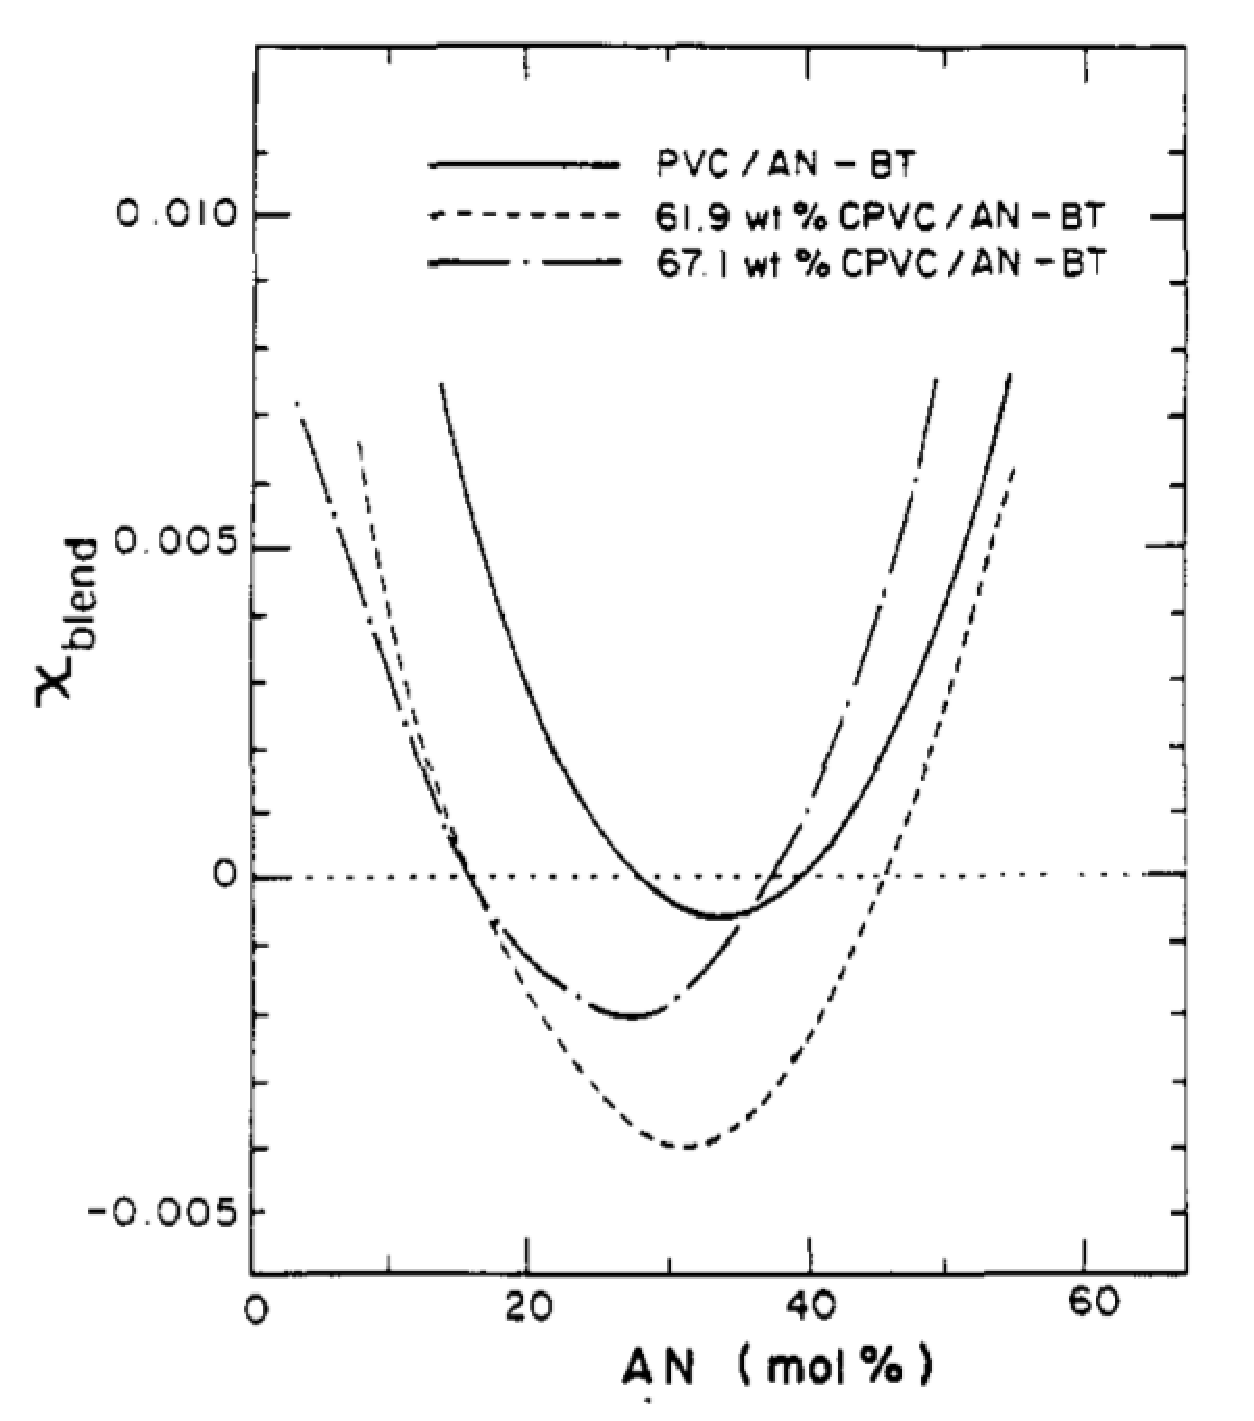
\includegraphics[width=.9\linewidth]{src/figure3.eps}
    \caption{计算了显示与 (AN-BT) 系统的混溶性窗口的功能的 CPVC/(AN-BT) 系统的 $chi_{blend}$}
    \centering
    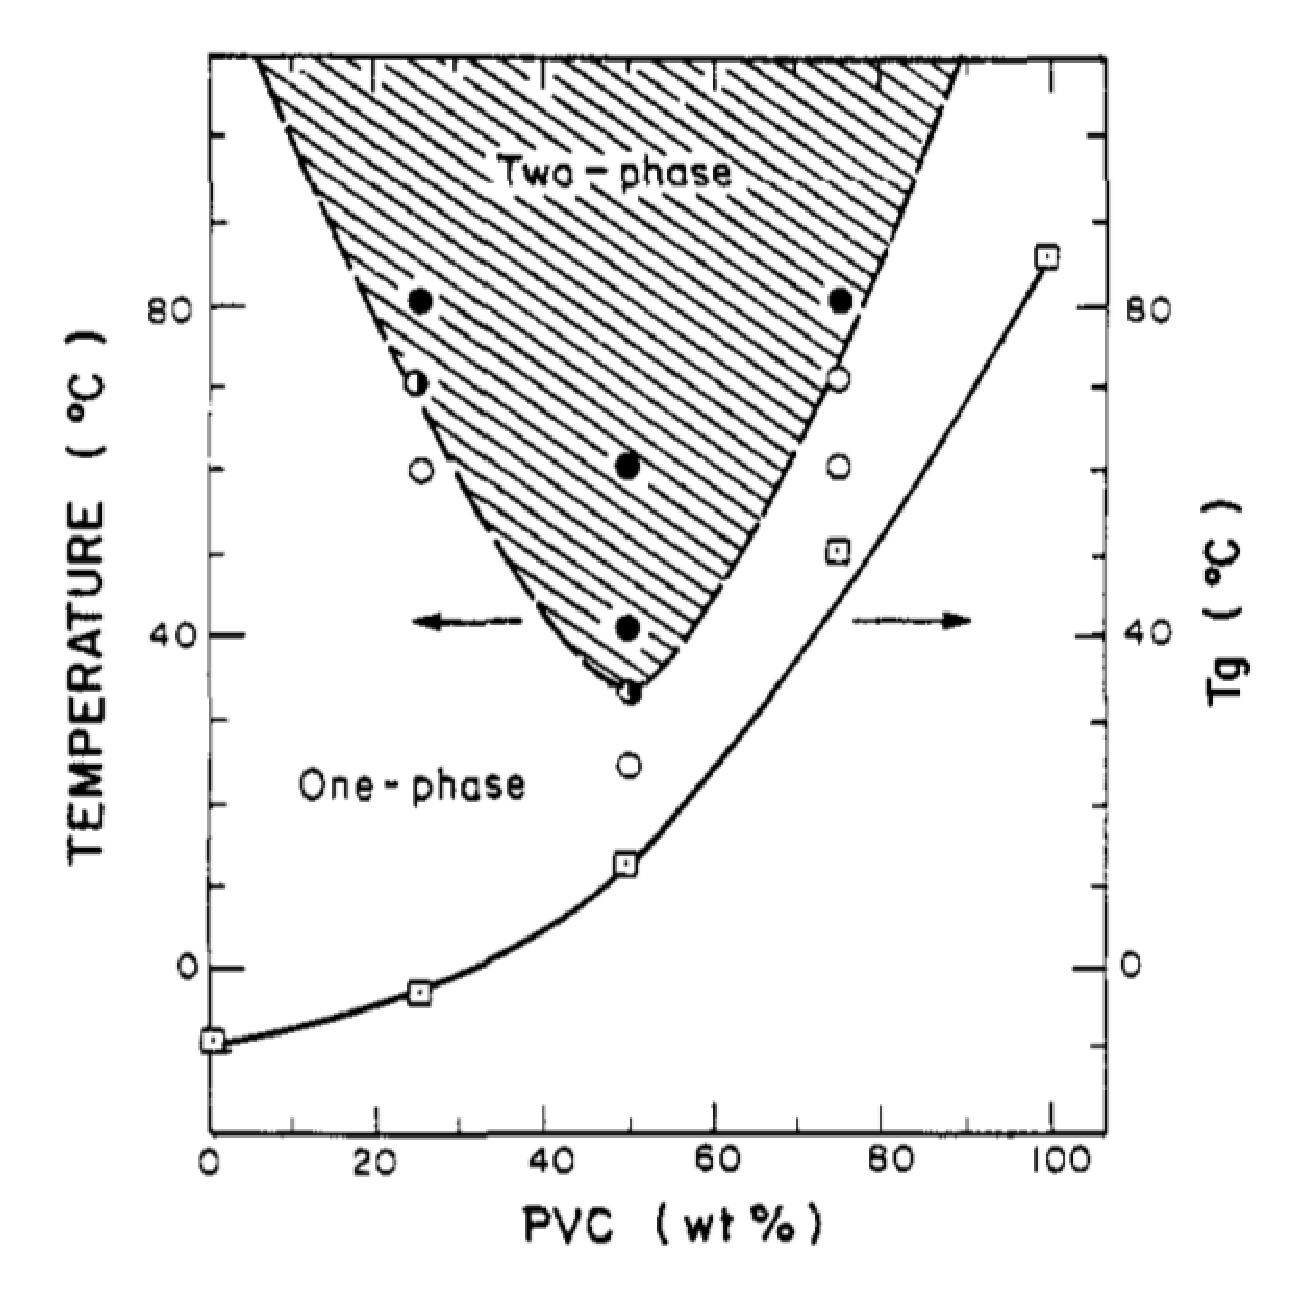
\includegraphics[width=.9\linewidth]{src/figure4.eps}
    \caption{PVC/(AN-BT) 系统的相图。半圆圈表示不明确的任务。还显示了各自共混物的 $T_g$} 
\end{figure}

对于 CPVC/(AN-BT) 系统,可以使用几个因素来解释增加的混溶性。混合窗口的扩展通过包含无规共聚物的共混物中的平均场理论来预测。由于每个无规共聚物中分子链段之间的排斥相互作用,与 PVC/(AN-BT) 体系中观察到的相比,混溶性窗口增加。在分子水平上,可以注意到,在 CPVC 中的 \chemfig{C-Cl} 和 (AN-BT) 中的 \chemfig{C~N} 之间存在诱导的偶极-偶极相互作用。随着 CPVC 中氯含量的增加,分子链段之间的偶极相互作用数量增加,这导致了混溶性窗口的扩大。当 CPVC 的氯含量在共混物中达到 63 wt\% CPVC 时,CHCl 与聚(AN-BT)AN 的 $\alpha$-H 的摩尔比接近最佳数目,达到有利的分子间相互作用,导致最大的混溶性。\par{}
高于该氯含量时,\chemfig{CCl_2} 单元的存在增加,并且与低氯含量的(AN-BT)无规共聚物相匹配的 CPVC 的显微组织开始随着 \chemfig{CCl_2} 单元数的增加而偏离。最终,高氯化物分子之间的相互作用较弱,可防止形成相互作用的分段相互作用,从而导致 CPVC 高氯含量下混溶性区域的收缩。\par{}
通过利用 ten Brinke 等人的平均场方法,可以分析该共聚物共聚物共混物的实验性相行为。根据方程 I,混合物 $\chi_{blend}$ 的总体相互作用参数可以表示为 $(A_{1-x}B_x)_n/(C_{1-y}D_y)_m$ 系统的分段相互作用参数的线性组合:
\begin{equation}
    \begin{aligned}
        \chi_{blend} = &(1-x)(1-y)\chi_{AC} + y(1-y)\chi_{AD} + \\
                        &x(1-y)\chi_{BC} + xy\chi_{BD} -    \\
                        &x(1-x)\chi_{AB} - y(1-y)\chi_{CD}
    \end{aligned}
\end{equation}

\begin{figure}[htb]
    \centering
    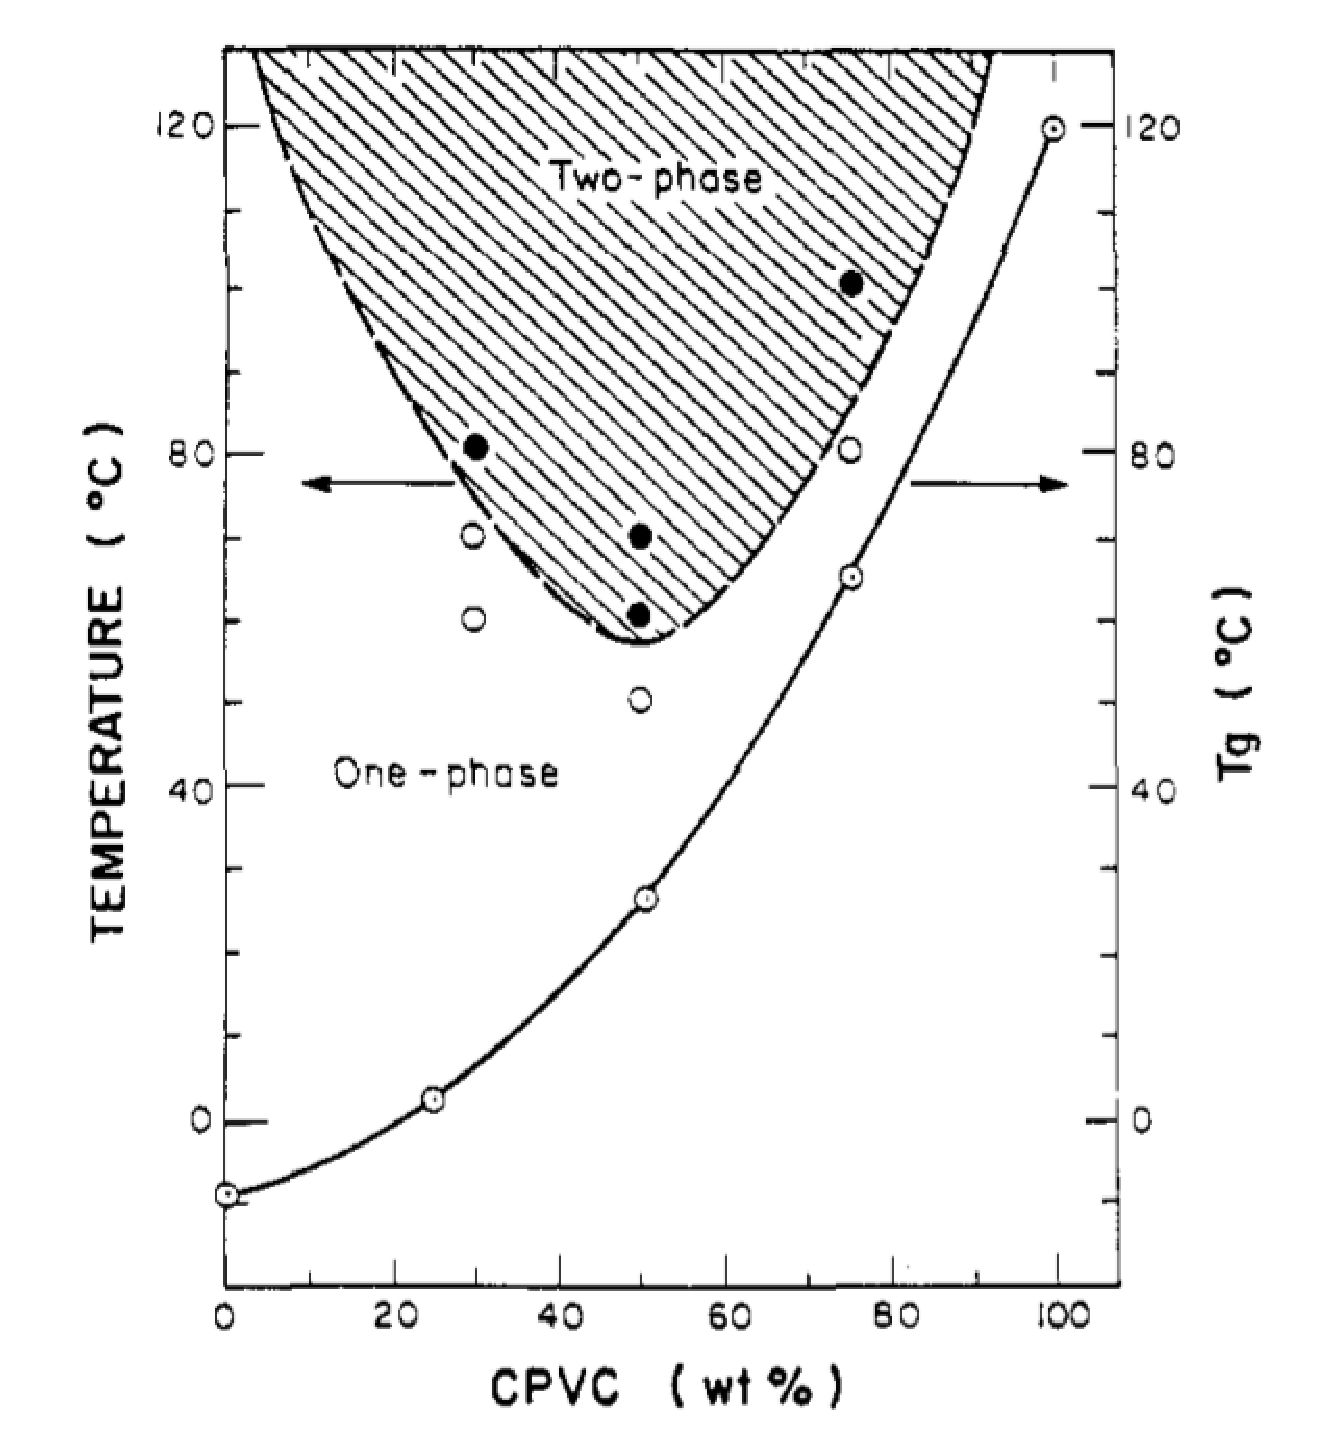
\includegraphics[width=.9\linewidth]{src/figure5.eps}
    \caption{64.2 wt\% CPVC/(AN-BT) 系统的相图。还显示了各自共混物的 $T_g$}
    \centering
    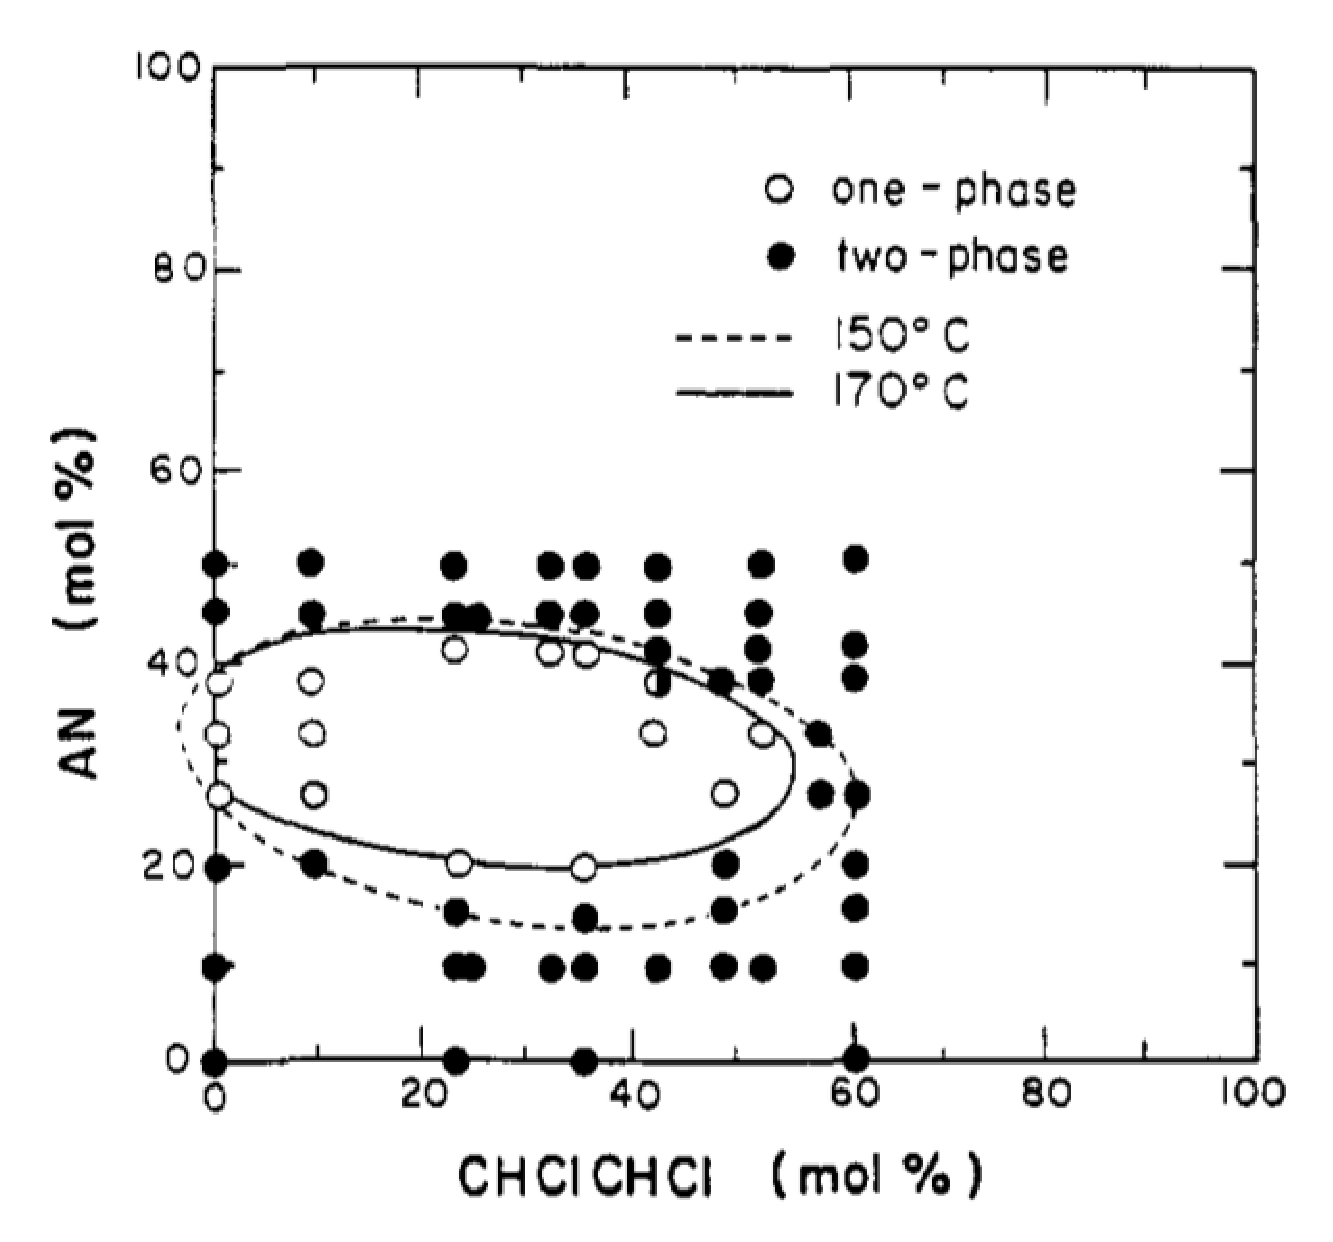
\includegraphics[width=.9\linewidth]{src/figure6.eps}
    \caption{在 170\cdegree 下 CPVC/(AN-BT) 共混物的等温混溶性-不混溶性图。半个圆圈表示不明确的任务。图 2 所示的混合窗口(虚线)已经叠加在图上,以便于在 150 和 170\cdegree 之间比较窗口尺寸}
\end{figure}

在这个表达式中,六个交互参数 $\chi_{ij}$'s 可以带符号,但通常是正的。当 $\chi_{AB}$ 和 $\chi_{CD}$ 足够大时,$\chi{blend}$ 可以是负的,并且在某些共聚物组成范围内可发生混溶。这可以被认为是在给定的共聚物链上的两个不同的共价连接的链段之间的排斥效应。在通常的 Flory-Huggins 表示中,临界点发生在 $\chi_{crit}$ 等于 \chemfig{CCl_2} 的温度下,其中
\begin{equation}
    \begin{aligned}
        \chi_{blend} = \frac{1}{2}(m^{-1/2}+n^{-1/2})^2
    \end{aligned}
\end{equation}

在目前的 CPVC/(AN-BT) 系统中,$\chi_{crit}$ 是从已知的聚合度计算的 0.001。表示 \chemfig{CH_2CHCl} 和 CHClCHCl 单元之间的相互作用的 $\chi_{AB}$ 是从 Shiomi 的实验数据获得的。 通过将实验混溶性-不混溶性边界拟合到平均场方程来计算剩余的 $\chi_{ij}$'s。代表该边界的图 II 中的虚线是平均场理论所要求的椭圆形形状。对于这个椭圆的具体方程式是:
\begin{equation}
    \begin{aligned}
        F(x, y) = &0.042x^2 + 0.1827y^2 - 0.0399x - \\
                  &0.1243y + 0.0491xy + 0.0204
    \end{aligned}
\end{equation}

边界条件由 $F(x, y) = \chi_{blend} - \chi_{crit} = 0$ 给出。二次广义方程的所有常数与 $\chi_{ij}$'s 直接相关。从实验确定的相边界(方程 4),计算相互作用参数,并列于表 II。通过利用这些相互作用参数值,CPVC/(AN-BT) 混合物中的混溶性区域可以基于平均场理论(方程 2 和 3)进行重建。\par{}
对于几种 CPVC 共混物计算了 CPVC/(AN-BT) 系统的 $\chi_{blend}$,并显示为图 3 中 AN 含量的函数。因为 CPVC 中可用的 $\alpha$-氢的数量的减少,存在于高氯化 PVC 中的 \chemfig{CCl_2} 单元可能影响丙烯腈和 CHClCHCl 之间的相互作用。因此,混合窗口中的最大值出现在 23 mol\% CHClCHCl(CPVC 中为63 wt\% Cl)的范围内;在较高的氯含量下,混溶性窗口的宽度减小,如图 3 所示,曲线表示较小的混溶区域。\par{}
共混物的相行为取决于温度以及两种共混组分的组成。图 4 显示了含有 44 mol\% (AN-BT) 的 PVC/(AN-BT) 共混物的相图。在整个组成范围内观察到单一玻璃化转变。随着温度的升高,系统逐渐相分离,观察到较低的临界互溶温度表现。这个结果与 Yoon 等人的研究一致。可以看出,LCST 处在 30\cdegree 附近。因此,如果在样品制备期间高温除去溶剂,结果将使样品相分离。\par{}

为了理解含共聚物的共混物的相行为的组成依赖性,构建了 64.2 wt\% CPVC/44 mol\% (AN-BT) 共混物的相图(图 5)。观察到图 4 所示的相同行为,而 LCST 发生在 55\cdegree 左右,增加了 20\cdegree,这直接证明可以通过改变共混物的化学成分来控制 LCST。\par{}
在显示 LCST 行为的系统中,预期当温度升高时,混溶性区域的尺寸减小。因此,在 170\cdegree 下,CPVC/(AN-BT)系统的混溶性-不混溶相图被示为图 6 中的实线。当与 150\cdegree(虚线)处的相边界相比时,混溶性区域减小。当温度升至 170\cdegree 时,在 150\cdegree 附近的临界边界周围的一些混溶混合物变得不混溶。可以看出,降低的混溶性区域有些不对称,代表高氯含量的组分的区域受温度升高的影响。\par{}
通过使用如上所述的几何分析和平均场方法,可以通过假设 150\cdegree 下的 $\chi_{AC}$ 与 170\cdegree 下的相同参数 $\chi_{ij}$'s 相同,来计算 170\cdegree 下的相互作用参数 $\chi_{ij}$'s。因为在 150 和 170\cdegree 下相似的混溶窗,证明 PVC 和聚丁二烯组分之间的相互作用参数 $\chi_{AC}$ 受到最小的影响。170\cdegree 下计算的 $\chi_{ij}$'s 在表11中示出。当与 150\cdegree 下的 $\chi_{ij}$'s 相比时,相互作用参数几乎相同,可以说上述假设对于该计算是合理的。\par{}

\section{结论}
CPVC/(AN-BT) 混合物显示出比 PVC/(AN-BT) 共混体系更宽的混溶性窗口;在 CPVC/(AN-BT) 共混物中,在 63 wt\% 能够观察到最大的混溶窗。通过研究温度对相位行为的影响,发现两种系统,PVC/(AN-BT) 和 CPVC/(AN-BT)都显示 LCST 现象。发现与 PVC/(AN-BT) 系统相比,CPVC/(AN-BT)系统的 LCST 得到提高。平均场方法提供了共聚物共聚物共混物的相组成图的令人满意的解释。


\end{document}
